% =====================================================================
%  Лекция 7. Методы построения точечных оценок: метод моментов,
%  метод максимального правдоподобия
%  Дата: 2026-10-29
% =====================================================================
\section[Метод моментов. Метод максимального правдоподобия]%
  {Методы построения точечных оценок: метод моментов,
   метод максимального правдоподобия}
\label{lec:07}

В лекции~\ref{lec:06} мы обсуждали, какими свойствами должна обладать хорошая оценка.
Теперь~--- как оценки строить. Всюду ниже $\xi$~--- генеральная совокупность с функцией
распределения $F_\xi(x, \theta)$, $\theta \in \Th$, и $X_{[n]} = (X_1, \ldots, X_n)$~--- выборка.

\subsection{Метод моментов}
\label{lec07:moments}

Сначала пусть параметр одномерный: $\theta \in \Th \subset \R$.

Идея: теоретическую характеристику распределения, которая зависит от~$\theta$, приравнять
к её выборочному аналогу и решить получившееся уравнение относительно~$\theta$.

Возьмём борелевскую функцию $g \colon \R \to \R$ и положим
\[
  m(\theta) = \int_{-\infty}^{+\infty} g(x)\, dF_\xi(x, \theta) = \E_\theta\, g(\xi).
\]
Её выборочный аналог получается заменой $F_\xi$ на эмпирическую функцию распределения:
\[
  \bar g = \int_{-\infty}^{+\infty} g(x)\, dF_n^*(x) = \frac1n \sum_{i=1}^n g(X_i).
\]
Составим уравнение
\begin{equation}
  \label{lec07:eq:mm}
  m(\theta) = \bar g.
\end{equation}

\begin{definition}
  Если уравнение~\eqref{lec07:eq:mm} имеет единственное решение $\hat\theta(X_{[n]})$, то есть
  функция~$m$ обратима, то
  \[
    \hat\theta(X_{[n]}) = m^{-1}(\bar g) = m^{-1}\biggl(\frac1n \sum_{i=1}^n g(X_i)\biggr)
  \]
  называется \emph{оценкой параметра~$\theta$, полученной методом моментов}.
\end{definition}

Название связано с тем, что обычно берут $g(x) = x^k$: тогда $m(\theta) = a_k$~---
теоретический момент, а $\bar g = a_k^*$~--- выборочный. Чаще всего $g(x) = x$, и
уравнение~\eqref{lec07:eq:mm} принимает вид $\E_\theta\,\xi = \Xbar$.

\subsubsection{Свойства оценок метода моментов}

Обозначим $h = m^{-1}$. Тогда
\[
  \hat\theta = h\biggl(\frac1n \sum_{i=1}^n g(X_i)\biggr)
\]
~--- это статистика первого типа (раздел~\ref{lec03:first-type}) с функциями $g$ и~$h$.
Точка, в которой <<работает>> $h$:
\[
  a = \E g(\xi) = m(\theta), \qquad h(a) = m^{-1}\bigl(m(\theta)\bigr) = \theta.
\]

\begin{enumerate}
  \item \textbf{Сильная состоятельность.} Если $h = m^{-1}$ непрерывна (в точке $a = m(\theta)$),
        то по теореме~\ref{lec03:first-type-conv}
        \[
          \hat\theta \toas h(a) = \theta,
        \]
        то есть оценка метода моментов сильно состоятельна.
  \item \textbf{Асимптотическая нормальность.} Пусть $m'(\theta) \ne 0$ и $\D g(\xi) < \infty$.
        По теореме о производной обратной функции
        \[
          h'(a) = \bigl(m^{-1}\bigr)'(a) = \frac{1}{m'(\theta)}.
        \]
        По теореме~\ref{lec04:first-type-limit-thm} (пункт~1, одномерный случай)
        \[
          \sqrt{n}\,(\hat\theta - \theta) = \sqrt{n}\,\bigl(S(X_{[n]}) - h(a)\bigr)
          \tod h'(a)\, \zeta, \qquad \zeta \sim \Norm\bigl(0, \D g(\xi)\bigr).
        \]
        Величина $h'(a)\,\zeta$ нормальна с нулевым средним и дисперсией $(h'(a))^2 \D g(\xi)$, поэтому
        \[
          \sqrt{n}\,(\hat\theta - \theta) \tod \Norm\biggl(0, \frac{\D g(\xi)}{(m'(\theta))^2}\biggr),
        \]
        то есть оценка асимптотически нормальна с коэффициентом
        $\sigma^2(\theta) = \dfrac{\D g(\xi)}{(m'(\theta))^2}$.
\end{enumerate}

\begin{reminder}[Теорема о предельном распределении статистик первого типа, одномерный случай]
  Пусть $S(X_{[n]}) = h\bigl(\frac1n \sum g(X_i)\bigr)$, $g, h \colon \R \to \R$ борелевские,
  $a = \E g(\xi)$, $\zeta \sim \Norm(0, \D g(\xi))$. Тогда
  \begin{enumerate}
    \item если существует $h'(a)$, то $\sqrt{n}\,\bigl(S(X_{[n]}) - h(a)\bigr) \tod h'(a)\,\zeta$;
    \item если $h'(a) = 0$ и существует $h''(a)$, то
          $n\,\bigl(S(X_{[n]}) - h(a)\bigr) \tod \frac12\, h''(a)\,\zeta^2$.
  \end{enumerate}
  (Теорема~\ref{lec04:first-type-limit-thm}.)
\end{reminder}

\subsubsection{Многомерный параметр}

Пусть $\theta = (\theta_1, \ldots, \theta_m) \in \Th \subset \R^m$. Тогда берут
$m$ функций, обычно степенных:
\[
  g(x) = \bigl(g_1(x), \ldots, g_m(x)\bigr) = (x, x^2, \ldots, x^m),
\]
и приравнивают первые $m$ теоретических моментов к выборочным:
\[
  \begin{cases}
    a_1(\theta) = a_1^*, \\
    \quad\vdots \\
    a_m(\theta) = a_m^*,
  \end{cases}
  \qquad a_k(\theta) = \E_\theta\, \xi^k, \quad a_k^* = \frac1n \sum_{i=1}^n X_i^k.
\]
Решение этой системы относительно $\theta_1, \ldots, \theta_m$ и есть оценка метода моментов.

\subsubsection{Примеры}

\begin{example}[нормальное распределение]
  \label{lec07:ex:mm-normal}
  $\xi \sim \Norm(a, \sigma^2)$, $\theta = (a, \sigma^2) \in \R \times (0, +\infty)$.
  Параметров два, берём $g(x) = (x, x^2)$. Так как $\D\xi = \E\xi^2 - (\E\xi)^2$,
  то $\E\xi^2 = \sigma^2 + a^2$. Система:
  \[
    \begin{cases}
      \E\xi = a_1^*, \\
      \E\xi^2 = a_2^*,
    \end{cases}
    \qquad\text{то есть}\qquad
    \begin{cases}
      a = \Xbar, \\
      \sigma^2 + a^2 = a_2^*.
    \end{cases}
  \]
  Выборочный аналог той же формулы для дисперсии:
  \[
    s^2 = \frac1n \sum_{i=1}^n (X_i - \Xbar)^2 = \frac1n \sum_{i=1}^n X_i^2 - \Xbar^2
        = a_2^* - \Xbar^2,
  \]
  то есть $a_2^* = s^2 + \Xbar^2$. Отсюда
  \[
    \hat a = \Xbar, \qquad \hat\sigma^2 = s^2.
  \]
  Заметим, что $\hat\sigma^2 = s^2$ смещена (пример~\ref{lec06:ex:var}): метод моментов
  несмещённости не гарантирует.
\end{example}

\begin{example}[показательное распределение]
  \label{lec07:ex:mm-exp}
  $\xi \sim \Exp(\lambda)$, $\theta = \lambda > 0$; $\E\xi = \frac1\lambda$,
  $\D\xi = \frac{1}{\lambda^2}$.

  \emph{Способ~1: $g(x) = x$.} Уравнение $\frac1\lambda = \Xbar$, откуда
  \[
    \hat\lambda = \frac{1}{\Xbar}.
  \]
  Её коэффициент асимптотической нормальности: $m(\lambda) = \frac1\lambda$,
  $m'(\lambda) = -\frac{1}{\lambda^2}$, $\D g(\xi) = \D\xi = \frac{1}{\lambda^2}$, поэтому
  \[
    \sigma^2(\lambda) = \frac{\D g(\xi)}{(m'(\lambda))^2} = \frac{1/\lambda^2}{1/\lambda^4} = \lambda^2.
  \]

  \emph{Способ~2: $g(x) = x^2$.} Теперь $m(\lambda) = \E\xi^2 = \D\xi + (\E\xi)^2
  = \frac{1}{\lambda^2} + \frac{1}{\lambda^2} = \frac{2}{\lambda^2}$, и уравнение
  \[
    \frac{2}{\lambda^2} = a_2^* = s^2 + \Xbar^2
    \qquad\Longrightarrow\qquad
    \hat\lambda = \sqrt{\frac{2}{s^2 + \Xbar^2}}.
  \]
  Выбор $g$ влияет на результат: разные~$g$ дают разные оценки одного и того же параметра.
\end{example}

\begin{example}[равномерное распределение]
  \label{lec07:ex:mm-unif}
  $\xi \sim \Unif[0, \theta]$, $\theta > 0$; $g(x) = x$. Так как $\E\xi = \frac\theta2$,
  уравнение $\frac\theta2 = \Xbar$ даёт
  \[
    \hat\theta = 2\Xbar.
  \]
\end{example}

\begin{example}[распределение Пуассона]
  $\xi \sim \Pois(\alpha)$: $\P\{\xi = k\} = \frac{\alpha^k}{k!} e^{-\alpha}$, $k = 0, 1, \ldots$
  Берём $g(x) = x$; $\E\xi = \alpha$, поэтому $\hat\alpha = \Xbar$.
\end{example}

\begin{example}[биномиальное распределение]
  $\xi \sim \Bin(N, p)$, число испытаний~$N$ известно, оценивается $p$.
  Берём $g(x) = x$; $\E\xi = Np$, уравнение $Np = \Xbar$ даёт
  \[
    \hat p = \frac{\Xbar}{N}.
  \]
\end{example}

\subsection{Метод максимального правдоподобия}
\label{lec07:mle}

Пусть сначала генеральная совокупность имеет плотность $f_\xi(x, \theta)$. Элементы выборки
независимы и распределены как~$\xi$, поэтому совместная плотность выборки равна
произведению плотностей:
\[
  f_{X_{[n]}}(x_1, \ldots, x_n; \theta) = \prod_{i=1}^n f_\xi(x_i, \theta).
\]

\begin{definition}
  \emph{Функцией правдоподобия} выборки $X_{[n]}$ называется
  \begin{itemize}
    \item если $\xi$ имеет плотность $f_\xi(x, \theta)$:
          \[
            L(X_{[n]}, \theta) = \prod_{i=1}^n f_\xi(X_i, \theta);
          \]
    \item если $\xi$ дискретна с возможными значениями $z_1, z_2, \ldots$ и вероятностями
          $p_k(\theta) = \P\{\xi = z_k; \theta\}$, $\sum_k p_k(\theta) = 1$:
          \[
            L(X_{[n]}, \theta) = \prod_{i=1}^n \P\{\xi = X_i; \theta\}.
          \]
  \end{itemize}
\end{definition}

Функцию правдоподобия рассматривают как функцию \emph{параметра}~$\theta$ при фиксированной
выборке. В дискретном случае смысл особенно нагляден: по независимости
\[
  L(X_{[n]}, \theta) = \P\{\xi = X_1; \theta\} \cdot \ldots \cdot \P\{\xi = X_n; \theta\}
\]
~--- это вероятность получить именно ту выборку, которая наблюдалась, если параметр
равен~$\theta$.

\begin{definition}
  \emph{Оценкой максимального правдоподобия} (ОМП) параметра~$\theta$ называется
  \[
    \hat\theta(X_{[n]}) = \argmax_{\theta \in \Th} L(X_{[n]}, \theta)
  \]
  (если максимум существует и достигается в единственной точке).
\end{definition}

Идея: в качестве оценки берём то значение параметра, при котором наблюдённая выборка
<<наиболее правдоподобна>>.

На практике удобнее максимизировать $\ln L$: логарифм строго возрастает, поэтому
$\argmax L = \argmax \ln L$, а произведение под логарифмом превращается в сумму.
Если $L$ дифференцируема по~$\theta$, точку максимума ищут среди решений \emph{уравнения
правдоподобия}
\[
  \frac{\partial \ln L(X_{[n]}, \theta)}{\partial \theta} = 0
\]
(для векторного $\theta$~--- система по всем компонентам), а затем проверяют, что это
действительно максимум. Уравнение правдоподобия~--- лишь необходимое условие
экстремума.

\begin{proposition}[инвариантность ОМП; {\cite[гл.~15, §2]{bure}}]
  \label{lec07:invariance}
  Пусть $\phi$~--- взаимно однозначное отображение множества $\Th$ на множество~$B$.
  Если $\hat\theta$~--- ОМП параметра~$\theta$, то $\phi(\hat\theta)$~--- ОМП параметра
  $\phi(\theta)$, и наоборот.
\end{proposition}

\begin{proof}
  Как функция нового параметра $b = \phi(\theta)$ правдоподобие равно
  $L\bigl(X_{[n]}, \phi^{-1}(b)\bigr)$. Оно принимает те же значения, что и
  $L(X_{[n]}, \theta)$, только <<с переобозначенным аргументом>>, поэтому максимум
  достигается при $\phi^{-1}(b) = \hat\theta$, то есть при $b = \phi(\hat\theta)$.
\end{proof}

Например, если $\hat\theta$~--- ОМП дисперсии, то $\sqrt{\hat\theta}$~--- ОМП среднеквадратичного
отклонения. Поэтому неважно, по какому из параметров $\sigma$ или $\sigma^2$ дифференцировать
в примере ниже.

\subsubsection{Примеры}

\begin{example}[нормальное распределение]
  \label{lec07:ex:mle-normal}
  $\xi \sim \Norm(a, \sigma^2)$, $\theta = (a, \sigma)$,
  $f_\xi(x, \theta) = \frac{1}{\sqrt{2\pi}\,\sigma} e^{-\frac{(x - a)^2}{2\sigma^2}}$.
  Функция правдоподобия и её логарифм:
  \begin{gather*}
    L(X_{[n]}, \theta) = \frac{1}{(2\pi)^{n/2} \sigma^n}
                         \exp\biggl(-\sum_{i=1}^n \frac{(X_i - a)^2}{2\sigma^2}\biggr), \\
    \ln L(X_{[n]}, \theta) = -\frac n2 \ln 2\pi - n \ln\sigma
                             - \sum_{i=1}^n \frac{(X_i - a)^2}{2\sigma^2}.
  \end{gather*}
  Приравниваем частные производные к нулю:
  \[
    \frac{\partial \ln L}{\partial a} = \frac{1}{\sigma^2} \sum_{i=1}^n (X_i - a) = 0,
    \qquad
    \frac{\partial \ln L}{\partial \sigma} = -\frac{n}{\sigma}
      + \frac{1}{\sigma^3} \sum_{i=1}^n (X_i - a)^2 = 0.
  \]
  Из первого уравнения $a = \Xbar$; подставляя во второе, $n\sigma^2 = \sum_{i=1}^n (X_i - \Xbar)^2$.
  Итак,
  \[
    \hat a = \Xbar, \qquad \hat\sigma^2 = \frac1n \sum_{i=1}^n (X_i - \Xbar)^2 = s^2
  \]
  ~--- те же оценки, что и у метода моментов (пример~\ref{lec07:ex:mm-normal}).
  Мы дифференцировали по~$\sigma$, а ответ записали для $\sigma^2$: это законно по
  инвариантности ОМП (утверждение~\ref{lec07:invariance}).
\end{example}

\begin{example}[равномерное распределение]
  \label{lec07:ex:mle-unif}
  $\xi \sim \Unif[0, \theta]$: $f_\xi(x, \theta) = \frac1\theta$ при $x \in [0, \theta]$
  и $0$ иначе. Произведение плотностей равно $\frac{1}{\theta^n}$, если \emph{все}
  $X_i \in [0, \theta]$, и нулю, если хотя бы одно $X_i \notin [0, \theta]$.
  Все $X_i \le \theta$ равносильно $X_{(n)} = \max_i X_i \le \theta$, поэтому
  \[
    L(X_{[n]}, \theta) =
    \begin{cases}
      0,                  & \theta < X_{(n)}, \\
      \dfrac{1}{\theta^n}, & \theta \ge X_{(n)}.
    \end{cases}
  \]
  На $[X_{(n)}, +\infty)$ функция $\frac{1}{\theta^n}$ убывает (\cref{lec07:fig:unif-L}),
  поэтому максимум достигается в левом конце:
  \[
    \hat\theta = X_{(n)} = \max_{1 \le i \le n} X_i.
  \]
  Здесь $L$ разрывна в точке максимума, и уравнение правдоподобия не помогает:
  максимум ищется непосредственно.
\end{example}

\begin{figure}[h]
  \centering
  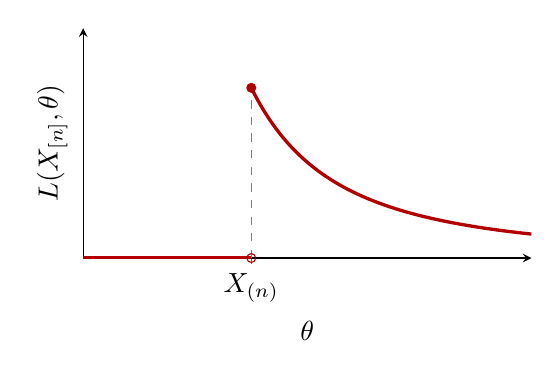
\begin{tikzpicture}
    \begin{axis}[
      width=0.6\textwidth, height=4.5cm,
      xmin=0, xmax=4, ymin=0, ymax=0.6,
      axis lines=left, xlabel={$\theta$}, ylabel={$L(X_{[n]}, \theta)$},
      xtick={1.5}, xticklabels={$X_{(n)}$},
      ytick=\empty,
    ]
      \addplot[very thick, red!70!black, domain=0:1.5, samples=2] {0};
      \addplot[very thick, red!70!black, domain=1.5:4, samples=80] {1/x^2};
      \addplot[only marks, mark=*, mark size=1.6pt, red!70!black] coordinates {(1.5, 0.4444)};
      \addplot[only marks, mark=o, mark size=1.6pt, red!70!black] coordinates {(1.5, 0)};
      \draw[dashed, gray] (axis cs:1.5,0) -- (axis cs:1.5,0.4444);
    \end{axis}
  \end{tikzpicture}
  \caption{Функция правдоподобия для $\Unif[0, \theta]$ (здесь $n = 2$): ноль левее $X_{(n)}$,
           убывающая $\theta^{-n}$ правее. Максимум~--- в точке $X_{(n)}$.}
  \label{lec07:fig:unif-L}
\end{figure}

\begin{example}[распределение Пуассона]
  \label{lec07:ex:mle-pois}
  $\xi \sim \Pois(\alpha)$, $\P\{\xi = k\} = \frac{\alpha^k}{k!} e^{-\alpha}$. Тогда
  \begin{gather*}
    L(X_{[n]}, \alpha) = \prod_{i=1}^n \frac{\alpha^{X_i}}{X_i!} e^{-\alpha}
      = \frac{\alpha^{\sum_i X_i}}{\prod_i X_i!}\, e^{-n\alpha}, \\
    \ln L(X_{[n]}, \alpha) = \ln\alpha \sum_{i=1}^n X_i - \ln \prod_{i=1}^n X_i! - n\alpha.
  \end{gather*}
  Уравнение правдоподобия:
  \[
    \frac{\partial \ln L}{\partial \alpha} = \frac{1}{\alpha} \sum_{i=1}^n X_i - n = 0
    \qquad\Longrightarrow\qquad
    \hat\alpha = \frac1n \sum_{i=1}^n X_i = \Xbar.
  \]
  Это максимум: $\dfrac{\partial^2 \ln L}{\partial \alpha^2} = -\dfrac{1}{\alpha^2} \sum_{i=1}^n X_i < 0$
  (если не все $X_i$ равны нулю).
\end{example}

\begin{addendum}
  Для $\Unif[0, \theta]$ два метода дают \emph{разные} оценки: $2\Xbar$ (метод моментов) и
  $X_{(n)}$ (ОМП). ОМП никогда не превосходит истинного~$\theta$ (все $X_i \le \theta$),
  а $2\Xbar$ может оказаться больше $\theta$ и даже меньше $X_{(n)}$~--- то есть
  противоречить самой выборке \cite[гл.~15, пример~2.2]{bure}.
\end{addendum}

\begin{keybox}[Что нужно знать к экзамену]
  \begin{itemize}
    \item Метод моментов: $m(\theta) = \E_\theta\, g(\xi)$, $\bar g = \frac1n \sum g(X_i)$,
          оценка $\hat\theta = m^{-1}(\bar g)$; многомерный случай~--- система на моменты.
    \item Свойства оценки метода моментов: сильная состоятельность (статистика первого типа,
          $h = m^{-1}$ непрерывна); асимптотическая нормальность с коэффициентом
          $\D g(\xi) / (m'(\theta))^2$ и откуда он берётся ($h'(a) = 1/m'(\theta)$).
    \item Примеры метода моментов: $\Norm(a, \sigma^2)$, $\Exp(\lambda)$ (двумя способами),
          $\Unif[0, \theta]$, $\Pois(\alpha)$, $\Bin(N, p)$.
    \item Функция правдоподобия (непрерывный и дискретный случаи), ОМП как $\argmax$;
          переход к $\ln L$; уравнение правдоподобия.
    \item Примеры ОМП: $\Norm(a, \sigma^2)$, $\Unif[0, \theta]$, $\Pois(\alpha)$.
  \end{itemize}
  \emph{Где легко ошибиться:}
  \begin{itemize}
    \item для $\Exp(\lambda)$ с $g = x^2$: $\E\xi^2 = 2/\lambda^2$, и
          $\hat\lambda = \sqrt{2/(s^2 + \Xbar^2)}$ (корень из всей дроби);
    \item в $\ln L$ для нормального закона $-\frac n2 \ln 2\pi$; производная по $\sigma$
          содержит $\sigma^3$ в знаменателе;
    \item для $\Unif[0, \theta]$ ОМП ищут без производной: $L$ разрывна, ответ $X_{(n)}$;
    \item ни метод моментов, ни ОМП не гарантируют несмещённости ($\hat\sigma^2 = s^2$).
  \end{itemize}
\end{keybox}
